\documentclass[10pt]{article}
\usepackage[final]{graphicx}
\usepackage{amsfonts}
\usepackage{amsmath}
\usepackage{caption}
\usepackage{subcaption}
\usepackage{url}
\usepackage{enumitem}
\usepackage{calc}
\usepackage{epstopdf}
\usepackage{float}

\topmargin-.5in
\textwidth6.6in
\textheight9in
\oddsidemargin0in

\def\ds{\displaystyle}
\def\d{\partial}

\begin{document}

\centerline{\large \bf Given a Helical Compression Spring in a Spring-Mass-Damper System, What are Optimal Springs?}

\vspace{.1truein}

\def\thefootnote{\arabic{footnote}}
\begin{center}
  
  Alistair Bentley\footnote{Mathematics, Clemson University},
   Tim Hodges\footnote{Mathematics, Colorado State University},
   Jiahua Jiang\footnote{Mathematics, University of Massachusetts Dartmouth },
  Justin Krueger\footnote{Mathematics, Virginia Tech},
  Saideep Nannapaneni\footnote{Civil \& Environmental Engineering,Vanderbilt University},
  Tianyu Qiu\footnote{Mathematics, University of Delaware}
   
\end{center}


%\vspace{.1truein}

\begin{center}
Problem Presenters: Jordan Massad\footnote{Sandia National Laboratory},
Sean Webb\footnote{Sandia National Laboratory};
	Faculty Mentors: Ilse Ipsen\footnote{Mathematics, North Carolina State University},
	Ralph Smith\footnote{Mathematics, North Carolina State University} 
\end{center}

%-----------------------------------------------------------------------Abstract-----------------------------------------------------------------------%
\vspace{.3truein}
\centerline{\bf Abstract}

The Helical compression spring is one of the most commonly used mechanical components in the world. As a result, spring design is a commonly performed task in industry and would benefit from the development of flexible tools that can answer the question of what make a spring design optimal would be beneficial. To address this, we develop an intelligent supporting tool using an object-oriented design framework that provides users the robustness needed to define and solve any spring design problem they require. In addition to our tool interfacing with a graphic user interface, we supplement its flexibility with analytic tools. One such tool provides global sensitivity analysis, and another provides a feasibility plot which helps the user determine if their problem has a solution or if it should be redefined. We also include a model for stress relaxation, which is a novel inclusion in the list of considerations for spring specifications. Both its unique flexibility and capability and the analytic tools we provide to support it make our tool useful in defining, solving, and analyzing optimal spring design problems. 

%-----------------------------------------------------------------------Introduction-----------------------------------------------------------------------%
\section{Introduction}
\label{sec:Introduction}

%-----------------------------------Introduction.1-----------------------------------%
\subsection{Acceleration Switch Example}
\label{subsec:Example}

Springs have many everyday uses, such as in cars, homes, gyms, and industry. For example, springs are used in acceleration switches like the one seen in Figure~\ref{fig:Acceleration_Switch}. Their purpose in this instance is to close an electrical circuit once the object carrying the switch reaches a certain acceleration. This mechanism provides power to sensory equipment and data recorders for very precise amounts of time, and an application of its use is to collect data from rocket sled experiments~\cite{Massad2015}. 
		\begin{figure}[H]
		 \begin{center}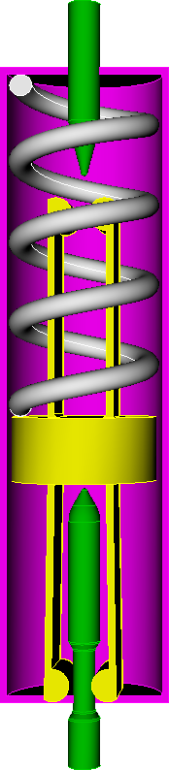
\includegraphics[scale=.2]{Acceleration_Switch.png}\end{center}
		 \caption{An example of an acceleration switch, see reference \cite{Massad2015}.}
		 \label{fig:Acceleration_Switch}		 
		 \end{figure}	 

These rocket sled tests include very high velocities and accelerations, and the experiments end with their destruction upon impact. Since the test is not easily replicated, we must have the ability to consistently and correctly collect data. This means we require that the spring in the acceleration switch must function as expected to the forces exerted on it, and having a switch that is closed earlier or later than expected is undesirable~\cite{IMSM2010}. Designing a spring to behave as desired is a complicated problem that requires satisfying numerous constraints on the spring's physical properties. That the desired spring can vary depending on the application further complicates the problem.

Spring design under these conditions amounts to a constrained optimization problem where certain properties of the spring may need to be maximized or minimized subject to bounds on some or all of the spring's other properties. Extending the scope beyond spring design for use in acceleration switches, which already cover a vast spread of specific spring designs, results in even more possibilities for design specifications. Rather than developing methods to solve these problems on an ad hoc basis, we develop to solve a wide variety of spring design problems. 

%-----------------------------------Introduction.2-----------------------------------%
\subsection{Optimal Spring Design}
\label{subsec:Spring Design} 

Designing an optimal spring is not a new problem. Brake et al. considered the design of an acceleration switch with enabled uncertainty~\cite{IMSM2010}. Alternatively, Sastry et al. implemented probabilistic response surface methodology to investigate the complications of uncertainty in designing a spring~\cite{Reliability}. Others have considered the reduction of the optimization problem to focus on a single parameter~\cite{Robust}. Similar tools to the ones mentioned above also exist~\cite{Paredes}.

Motivated by a workflow for the design process, we present an intelligent tool for building an optimal spring. This tool is robust to a variety of spring design specifications and allows for optimization under uncertainty. We promote user interactivity by interfacing our tool with a graphical user interface and providing a tool to visualize the feasibility of a spring design. We also provide the ability to perform a global sensitivity analysis with respect to a spring's design variables. Finally, we add stress relaxation as a optional specification for optimal spring design, which to our knowledge has never been included before. 

In this manuscript we provide details for our novel and robust tool as follows. Section~\ref{sec:The_Problem} formally defines the spring design problem for helical compression springs. Section~\ref{sec:The_Approach} outlines the workflow for optimal spring design. Section~\ref{sec:Computational_Experiments} shares cases studies using our approach, and Section~\ref{sec:Summary} summarizes our work and provides suggestions for future work.

%-----------------------------------------------------------------------The Problem-----------------------------------------------------------------------%		
\section{The Problem} 
\label{sec:The_Problem}

To develop the optimal spring design tool, we first need to identify and define the problem. This section explains the specific parameters and attributes relevant to optimal spring design, and then frames the optimization problem in a mathematical context.

%-----------------------------------The Problem.1-----------------------------------%
\subsection{Helical Compression Springs}
\label{sec:Springs}

Helical compression springs, such as the one in Figure~\ref{fig:Spring}, are possibly the most recognizable type of spring and are the spring of choice for this work. 
		\begin{figure}[H]
		 \begin{center}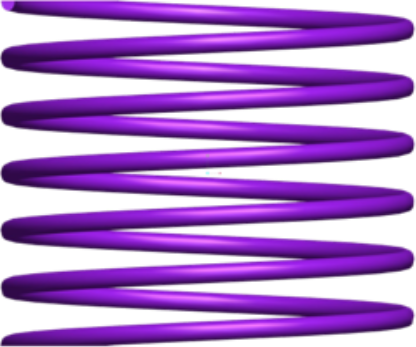
\includegraphics[scale=.2]{Spring.png}\end{center}
		 \caption{An example of a helical compression spring~\cite{Massad2015}.}
		 \label{fig:Spring}
		 \end{figure}
We can uniquely define a helical compression spring by a set of design parameters, which then determine physical attributes of the spring~\cite{Massad2015}. Figures~\ref{fig:Description1}~and~\ref{fig:Description2} provide visual representations for a few of the basic parameters, and a complete list of parameters. 		 
		\begin{figure}[H]
			\begin{subfigure}{.5\textwidth}
				\centering
				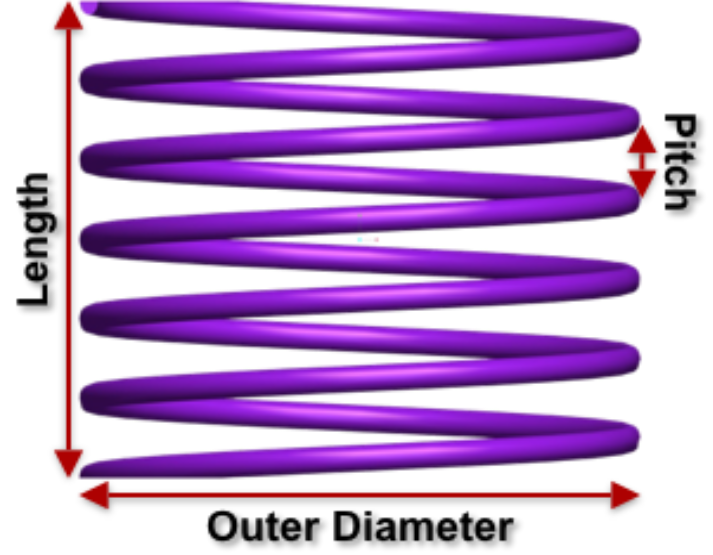
\includegraphics[scale=.17]{Spring_Description.png}
				\caption{The pitch, outer diameter, and length of a spring.}
				\label{fig:Description1}
			\end{subfigure}%
			\begin{subfigure}{.5\textwidth}
				  \centering
		 		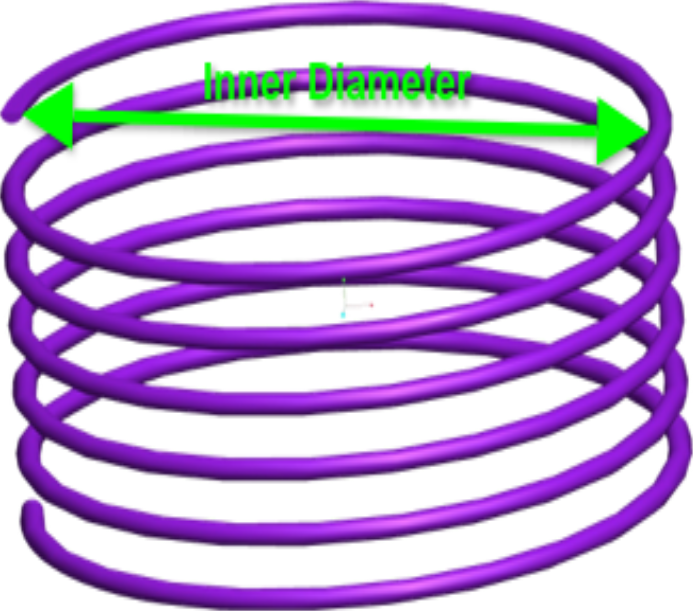
\includegraphics[scale=.155]{Spring_Description2.png}
				\caption{The inner diameter of a spring.}
				  \label{fig:Description2}
			\end{subfigure}
			 \label{fig:Descriptions}
		  \caption{A subset of basic parameters for a helical compression spring.}
		\end{figure}
		
		\begin{center}\textbf{Spring Design Parameters}\end{center}
		\begin{description}[leftmargin=!,labelwidth=\widthof{\bfseries Young's Modulus (E)}]
		
			\item [Wire Diameter ($\boldsymbol{d}_{\text{w}}$)] This is the diameter of the circular wire used to form the spring.
		
			\item [Inner Diameter ($\boldsymbol{d}_{i}$)] This is the diameter of the circle formed by the spring's interior excluding the wire. See Figure~\ref{fig:Description2}.
			
			\item [Outer Diameter ($\boldsymbol{d}_{\text{o}}$)] This is the diameter of the circle formed by the spring including the wire, so ${d_{\text{o}} = d_{\text{i}} + 2d_{\text{w}}}$. See Figure~\ref{fig:Description1}.
			
			\item[Total Coils ($\boldsymbol{N}_{\text{t}}$)] This is the total number of 360 degree rotations formed by the spring coil. The value does not have to be an integer. 
			
			\item[Active Coils ($\boldsymbol{N}_{\text{a}}$)] This is the number of coils that contribute to the force opposing any compression force on the spring. The number of active coils depends on $N_{t}$ and the spring's end conditions. If the end condition is \textit{closed} the terminal coils of the spring are welded to their adjacent coils and $N_{a} = N_{t}-2$. If the end condition is \textit{open}, the terminal coils of the spring are free and $N_{a} = N_{t}-1$. Note this relationship creates a lower bound on the total number of coils.

			\item[Free Length ($\boldsymbol{L}_{\text{free}}$)] This is the spring's length without any force acting on it, i.e., the spring's natural length.
						
			\item[Open Length ($\boldsymbol{L}_{\text{open}}$)] This is the spring's resting length in its application. In the acceleration switch, for example, it is the length of the spring in the switch when the switch is not in use. 
						
			\item[Hard Length ($\boldsymbol{L}_{\text{hard}}$)] This is the minimum length a spring can compress to under a specified force. For the acceleration switch example, the spring cannot compression beyond a certain point under the applied forces because additional compression would reopen the circuit.
			
			\item[Solid Length ($\boldsymbol{L}_{\text{solid}}$)] This is the spring's length when its coils are completely compressed. The solid length is $L_{\text{solid}} = N_{\text{t}}d_{\text{w}}$. Also, the lengths defined must satisfy ${L_{\text{solid}} \le L_{\text{hard}} < L_{\text{open}} \le L_{\text{free}}}$.
			
			\item[Deflection ($\boldsymbol{s}$)] This is the amount the spring is compressed.
					
			\item[Pitch ($\boldsymbol{p}$)] This is the distance between coils. For coils with \textit{closed} end conditions, ${p = \frac{L_{\text{free}}-2d_{\text{free}}}{N_{\text{a}}}}$, and for coils with \textit{open} end conditions, $p = \frac{L_{\text{free}}}{N_{\text{a}}-1}$. See Figure~\ref{fig:Description1}.			
			
			\item[Young's Modulus ($\boldsymbol{E}$)] This describes the spring's response to uniaxial stress and is one defining aspect of the spring's rigidity. Young's modulus is also know as the modulus of elasticity.
			
			\item[Poisson Ratio ($\boldsymbol{\nu}$)] This is a measurement of how much the spring deforms in any two dimensions when it is compressed in the third dimension.
			
			\item[Shear Modulus ($\boldsymbol{G}$)] This describes the spring's response to shear stress and is another defining aspect of the spring's rigidity. The shear modulus is also known as the modulus of rigidity and is $G = \frac{E}{2(1+\nu)}$. 
		
		\end{description}

This list of parameters is not exhaustive, but the parameter set given here defines many common spring attributes relevant to optimal spring design. We have a particular interest in the attributes listed below.

		\begin{center}\textbf{Spring Attributes}\end{center}
			\begin{description}
			
				\item [Spring Rate] \begin{equation} k = \frac{G}{8N_{\text{a}}}\frac{d_{\text{w}}^{4}}{(d_{\text{i}} + d_{\text{w}})^{3}}\end{equation}
				The spring rate measures the rigidity or stiffness of the spring. 
			
			\item[Spring Index]\begin{equation}C = \frac{d_{\text{i}}}{d_{\text{w}}} + 1\end{equation}
				The spring index measures the ratio between the spring's inner diameter and wire diameter and often is proportional to the manufacturing cost for the spring~\cite{SpringIndex}.
			
			\item[Preload Force]\begin{equation*} F_{\text{open}} = (L_{\text{free}}-L_{\text{open}})k = (L_{\text{free}}-L_{\text{open}})\frac{G}{8N_{\text{a}}}\frac{d_{\text{w}}^{4}}{(d_{\text{i}} + d_{\text{w}})^{3}} \end{equation*}
				Preload Force is the force applied to the spring while it is in the open position. For the acceleration switch example, this is the force applied on the spring when the switch is not in use.  
				
			\item[Coil Binding Gap]\begin{equation} g = \frac{L_{\text{hard}} - L_{\text{solid}}}{N_{\text{t}} - 1}\end{equation}		
				Coil binding gap is the pitch of the spring when the spring is compressed to its hard length. 
			 
			 \item[Buckling Slenderness Ratio]\begin{equation*} \lambda = \frac{L_{\text{free}}}{d_{\text{i}} + d_{\text{w}}} \end{equation*}
			 	The buckling slenderness ratio measures the spring's susceptibility to buckling under compression.
			 
			 \item[Maximum Shear Stress]\begin{equation} \tau = \frac{G(L_{\text{free}} - L_{\text{hard}})}{4 \pi N_{\text{a}}} \left[\frac{d_{\text{w}} (4d_{\text{i}}^{2} + 9.46d_{\text{i}} 
d_{\text{w}} + 3 d_{\text{w}}^{2})}{d_{\text{i}}(d_{\text{i}}+d_{\text{w}})^{3}}\right]\end{equation}
				This expression approximates the maximum shear stress applied to the spring. 
			
			\item[Diametral Expansion]\begin{equation} d_{\text{expand}} = d_{\text{w}} + \sqrt{(d_{\text{i}} + d_{\text{w}})^{2} + \frac{p^{2} - d_{\text{w}}}{\pi^{2}}}
			\end{equation}
				The diametral expansion is the measurement of how much the outer diameter of the spring increases as the spring is compressed. The discriminant of the square root is necessarily nonnegative, so diametral expansion can put additional constraints on the relationship between some parameters. Note also that the formula for diametral expansion depends on the spring's end conditions. The equation above is the diametral expansion of a spring with \textit{closed} end conditions, and the diametral expansion for a spring with \textit{open} end conditions is the solution of a cubic polynomial to complicated to show here.
						
			\item[Stress Relaxation]\begin{equation} \phi = \frac{2\pi N_{\text{a}} (d_{\text{i}}+d_{\text{w}})^2}{Gsd_{\text{w}}^4}\int_0^{d_\text{w}} r^2 \left(\left(\frac{2Gsr}{\pi N_{\text{a}} (d_{\text{i}}+d_{\text{w}})^2}\right)^{-n} + {c\over k} Gnt^k \right)^{-{1\over n}} \,\mathrm{d} r \end{equation}
				Stress relaxation measures how much the spring force decays in high temperature conditions under constant compression for time $t$. This model formula is derived using the Norton-Bailey law where $c$, $n$, and $k$ are temperature dependent material specific constants. The inclusion of stress relaxation as a spring attribute in optimal spring design is unique to our tool construction. We include a detailed derivation of this formula in Section~\ref{sec:Appendix}.
						
			\end{description}
			
Considering this list of spring parameters and attributes, optimal spring design amounts to optimizing a collection of parameters and attributes subject to the restrictions of design specifications. We formulate this objective as a constrained optimization problem.

%-----------------------------------The Problem.2-----------------------------------%
\subsection{Constrained Optimization}
\label{sec:Constrained_Optimization}

Given an input of objectives and constraints on those objectives which are both defined by a set of design variables, we can formulate the challenge of designing an optimal spring as a constrained optimization problem. Without loss of generality, the formulation of such a problem is
			\begin{equation}
				\begin{gathered}
	 				\min_{\mathbf{x}} \ F(\mathbf{x}) \\
	 				\mbox{subject to} \quad \mathbf{G}(\mathbf{x}) \le \mathbf{0}, 
				\end{gathered}
				\label{eq:General_Problem}	
			\end{equation}
Here, $\mathbf{x}$ is the set of independent variables for the problem. In the context of spring design the independent variables are the spring parameters, which we also call design variables in the context of optimization. The function $F(\mathbf{x})$ is the objective function that we try to optimize. For spring design this function can consist of a single spring attribute or any weighted linear combination of attributes. Lastly, the function $\mathbf{G}(\mathbf{x})$ is the set of constraint functions restricting the optimization problem. For spring design, this set can consist of any combination of bounds on the design variables and bounds on the spring attributes. 

To solidify this formulation, consider the acceleration switch example provided in the introduction. Suppose we wish to minimize the weighted sum of the spring rate ($k$) and the spring index ($c$) with respect to the inner diameter ($d_{\text{i}}$) and wire diameter ($d_{\text{w}}$) of the spring. Suppose we must satisfy a lower bound on the wire diameter ($d_{\text{w,min}}$), an upper bound on the inner diameter ($d_{\text{i,max}}$), and an additional constraint that the coil binding gap ($g$) is greater than the value $g_{\text{min}}$. Composing this problem mathematically gives
				\begin{equation}
 					\begin{gathered}
 						\min_{d_{\text{i}}, d_{\text{w}}} \ w_{1}k + w_{2}c \\
 						\mbox{subject to} \quad
						 \begin{split} 
						 	c - c_{\text{max}}\le 0, \\
						 	-d_{\text{w}} + d_{\text{w,min}}\le 0, \\
							d_{\text{i}} - d_{\text{i,max}} \le 0,
						\end{split}
					\end{gathered}
				\end{equation}
or equivalently,
 					\begin{equation}
 					\begin{gathered}
 						\min_{d_{\text{i}}, d_{\text{w}}} \ w_{1}\left(\frac{G}{8N_{\text{a}}}\frac{d_{\text{w}}^{4}}{(d_{\text{i}} + d_{\text{w}})^{3}}\right) + w_{2}\left(\frac{d_{\text{i}}}{d_{\text{w}}} + 1\right) \\ \\
 						\mbox{subject to} \quad
						 \begin{split} 
						 	-\frac{L_{\text{hard}} - L_{\text{solid}}}{N_{\text{t}} - 1} + g_{\text{min}}\le 0, \\
						 	-d_{\text{w}} + d_{\text{w,min}}\le 0, \\
							d_{\text{i}} - d_{\text{i,max}} \le 0,
						\end{split}
					\end{gathered}
					\label{eq:Problem}
				\end{equation}				
where $w_{1}$, $w_{2}$, $c_{\text{max}}$, $d_{\text{w,min}}$, $d_{\text{i,max}}$ are known values.

%-----------------------------------------------------------------------The Approach-----------------------------------------------------------------------%
\section{The Approach}
\label{sec:The_Approach}

Our approach follows the optimal spring design workflow illustrated in Figure~\ref{fig:Workflow}. This is an iterative process that receives a user specified problem, reformulates and solves the problem, and then returns a result for the user to accept or decline. The remainder of this section expands upon the details of each element in this diagram.
		\begin{figure}[H]
		 \begin{center}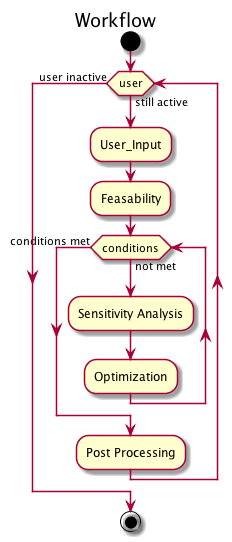
\includegraphics[scale=.4]{IMSM_Workflow.png}\end{center}
		 \caption{A workflow demonstrating the problem approach.}
		 \label{fig:Workflow}
		 \end{figure}

%-----------------------------------The Approach.1-----------------------------------%
\subsection{User Input}
\label{subsec:User_Input}

During the first step of our work flow, a spring designer (herein known as the user) presents an arbitrary spring design problem. For instance, the user might be interested in building a spring to use in the acceleration switch described in the introduction. Alternatively, the user might be interested in designing a spring for shock absorption on a car. During this initial phase, any spring used in an industrial application could be given as input.

%-----------------------------------The Approach.2-----------------------------------%
\subsection{Problem Definition}
\label{sec:Problem_Definition}

Generally, the user would like to optimize some of the spring attributes introduced in Section~\ref{sec:Springs}, while satisfying the problem's physical design constraints. In the case of an acceleration switch example in Section~\ref{sec:Constrained_Optimization}, the user would like to achieve the smallest possible weighted sum of spring rate ($k$) and spring index ($c$), while satisfying the physical dimensions of the spring and the constraint on the coil binding gap $g$. Thus, the next step in our workflow is to take the user input and formulate an optimization problem that includes an objective, a set of design variables and constraints. For the acceleration switch, this results in the problem defined in~(\ref{eq:Problem}). 

In order to run the design analysis, we place some restrictions on the form of this optimization problem. First, the optimization's objective function must be specified as a weighted sum of minimums and maximums. While other methods for multi-criteria optimization exist, including these in our scheme has been left to future work.

The second restriction, based on discussions with engineers experienced with spring design, is to reduce the set of design variables and optimization attributes to those in Table~\ref{tab:Design}.
\begin{table}
\caption{Variables and attributes that define a spring design.}
	\centering
	 \begin{tabular}{ c  c }
	 \hline\hline
	 Permissible Design Variables & Permissible Attributes for Optimization \\
	 \hline
     	The spring's natural length ($L_{\text{free}}$) 					& Spring Rate ($k$) \\
	    The spring's resting length ($L_{\text{open}}$) 				& Spring Index ($c$)  \\
		Spring's minimum compression length  ($L_{\text{hard}}$) 	& Preloaded Force ($F$) \\
		Total spring coil ($N_{\text{t}}$)    						& Coil Binding Gap ($g$) \\
		Spring's inner diameter ($d_{\text{i}}$)    					& Buckling Slenderness Ratio ($\lambda$) \\
		Spring's width diameter ($d_{\text{w}}$)    					& Shear Stress ($\tau$) \\
		Shear modulus  ($G$)        							& Diametral Expansion ($d_{\text{expand}}$) \\
														& Stress Relaxation ($\phi$) \\
														& Outer Diameter ($d_{\text{o}}$) \\
\hline\hline
	 \end{tabular}
	 \label{tab:Design}
\end{table}
The decision to limit the space of design variables and objective functions is not a limitation of this method.  Rather, it represents the set of options currently available in our design library.  If the user wishes to constrain or optimize an attribute that is not part of the existing library, the flexibility to add it is available.

An example of this flexibility is our team's integration of stress relaxation into the design process, which, to our knowledge, no other spring design system has. After our team found an acceptable mathematical formulation for stress relaxation as shown in~\ref{sec:Springs}, the function library was extended, allowing the user to incorporate relaxation into any problem formulation.

In addition to the design variable and spring attribute libraries, we employed an object-oriented approach to our software design to maximize the flexibility in our workflow. Object-oriented programming is an approach to software design that centers around classes, which are data containers capable of performing a predefined set of tasks. For example, our program has a \textit{Constraint} class that includes the constraint's function, and a way to determine if the constraint is violated at a given point. For a few examples of classes, see Figures~\ref{fig:Spring_Class}~and~\ref{fig:Objective_Constraint}. 
\begin{figure}[H]
			\begin{subfigure}{.5\textwidth}
				\centering
				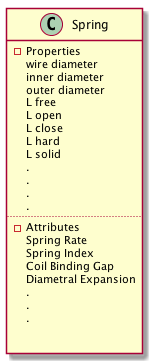
\includegraphics[scale=.5]{Spring_Class.png}
				\caption{\textit{Spring} class.}
				\label{fig:Spring_Class}
			\end{subfigure}%
			\begin{subfigure}{.5\textwidth}
				  \centering
		 		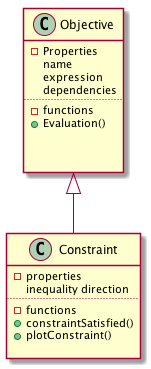
\includegraphics[scale=.5]{Objective_Constraint.png}
				\caption{\textit{Objective} and \textit{Constraint} classes.}
				  \label{fig:Objective_Constraint}
			\end{subfigure}
			 \label{fig:Classes}
		  \caption{Examples of classes.}
		\end{figure}
Using classes allow flexibility because the program's algorithm are designed to operate on the classes. For example, when the user inputs a new problem, the program generates an object with a specific objective function and set of constraints, and proceeds to use this object for the remainder of the program run time. Thus, our software can automatically convert the user problem into objects need for the optimizer to run.

%-----------------------------------The Approach.3-----------------------------------%
\subsection{Feasibility}
\label{subsec:Feasibility}

Once the user has set a problem, the next step is determining if a solution exists for the problem. This entails determining if there is a region in the space of design variables such that all the constraints defined in the problem are satisfied by points in this region. We call this region of interest the feasible region. Returning to the acceleration switch example, the feasible region is the region defined by the three constraints in~\ref{eq:Problem}, i.e., $-\frac{L_{\text{hard}} - L_{\text{solid}}}{N_{\text{t}} - 1} + g_{\text{min}}\le 0$, $-d_{\text{w}} + d_{\text{w,min}}\le 0$, and $d_{\text{i}} - d_{\text{i,max}} \le 0$. If the constraints are such that no feasible region exists, then the problem is poorly defined and the user should modify it. To assess feasibility, we use a Latin hypercube sampling method, which is designed to ensure sampling coverage over the entire domain. This approach is used because the user defined constraints are very general in nature, e.g., they can be linear or non-linear. 
Additionally, a graphical tool has been added to help the user analyze the problem's feasible region and the value of the objective function over the region. Using this tool, a plot with two or three state variables displays the problem's overall feasible region and the feasible region each individual constraint forms. This allows users to identify the nature of the constraints in their problem.

%-----------------------------------The Approach.4-----------------------------------%
\subsection{Optimization}
\label{subsec:Optimization}

\paragraph{Global Optimization} Without loss of generality, we can formulated a constrained design optimization problem as it is written in~(\ref{eq:General_Problem}). Several optimization algorithms (both local and global) are available to solve the above optimization problem. DIRECT is one of the most popular global search optimization algorithm~\cite{DirectUserGuide,DirectPaper} and is what we use this spring optimization problem.

The main idea of the DIRECT algorithm is that we normalize the domain to be a unit hypercube and evaluate the function at the center point $c$ of this hypercube and at points $\{c + \delta, c, c - \delta\}$ where $\delta$ is the size of the hypercube. Then we choose the hypercube that contains the smallest function value and further divide it into smaller hypercubes until we reach the global optimum. Because DIRECT is a sampling optimization algorithm, it requires no additional information from the objective function, such as its gradient or Hessian, and since it is a global algorithm, DIRECT does not require an initial point to begin optimization. Finally, DIRECT is easy to implement in an automated software framework since it does not require the segregation of linear and non-linear constraints.

\paragraph{Optimization Under Uncertainty} It is also essential to account for the variability in the manufacturing process, i.e., tolerances, in the design of springs. We also refer to tolerance as error or uncertainty in the design variables. The tolerance for each of the spring parameters is nominally assumed to be equal to one percent of the value of the variable. Thus, each variable has a uniform distribution with unknown mean and variance, which dependent on the mean value. The optimization formulation after accounting for tolerances can now be written as 
\begin{equation}
				\begin{gathered}
	 				\min_{\mathbf{x}} \ \mu_{F} (\mathbf{x},d) \\
	 				\mbox{subject to} \quad 
					\begin{split}
					-Pr(g_{i}(\mathbf{x},d) \leq 0) + p_{t}^{i} \le 0, \\
					-Pr(\mathbf{x} \geq lb_{\mathbf{x}}) + p_{lb} \le 0, \\
					-Pr(\mathbf{x} \leq ub_{\mathbf{x}}) + p_{ub} \le 0
					\end{split}
				\end{gathered}
			\end{equation}
where $\mathbf{x}$ and $d$ represent the design variables with tolerances and non-design variables with tolerances, respectively. The first constraint represents the probabilistic inequality constraint and the other constraints represent the bounds for the design variables. Optimization with tolerance is a nested double loop process where we carry out optimization in the outer loop, and in each iteration of optimization, we carry out reliability analysis in the inner loop using Monte Carlo sampling to check the probabilistic constraints. After obtaining the optimum values of the means of the design variables, we obtain their corresponding probability distributions since it is assumed that the variables follow uniform distributions with variances dependent on the mean values. 

Since the optimal design parameters are stochastic, the optimum value of the objective function, which is a function of the optimum design variables is also stochastic. We obtain the probability distribution of the optimum value objective function from the probability distributions of the design variables through uncertainty propagation analysis using Monte Carlo sampling. One random realization of each of the design parameters when passed through the objective function provides one realization of the optimum value of the objective function. Thus, we obtain several realizations of design variables, which result in several realizations of the optimum value of the objective function. Using the realizations, we use the Gaussian kernel density approach to construct the probability distribution.

%-----------------------------------The Approach.5-----------------------------------%
\subsection{Sensitivity Analysis}
\label{subsec:Sensitivity}
As the dimension of design variable space increases, the computational expense of the optimization procedure increases. To reduce the computational expense, we try to shrink the design variable space by removing the variables that have very little influence on the objective function. Thus, we require a dimension reduction strategy. Dimension reduction approaches have been divided into two categories, the filter approach~\cite{Bioinformatics} and the wrapper approach~\cite{Wrappers}. In the filter approach, we rank the input variables according to a ranking criterion, and we select the most dominant variables by assuming a threshold influence value. In the wrapper approach, we select a subset of variables from the list of all possible subsets of the input variables that best estimate the output variable. We use sensitivity analysis, a filter approach, in this work for dimension reduction. Two types of sensitivity analysis, local sensitivity analysis and global sensitivity analysis, have been developed in the literature. The local sensitivity index of a variable measures the sensitivity of the model output when the variable is fixed at a single value whereas the global sensitivity (GSA) index measures the variation of model output when the variable is varied over its range~\cite{Global}. We choose to use GSA as it considers the entire range instead of conditioning at a point in computing the sensitivity to the output. Note that the input variables represent the design variables and model represents the objective function.
Consider an objective function, $F$ with $n$ design variables $x_{1}$, $x_{2}$, ...  $x_{n}$ given by
\begin{equation}
Y = F(x_{1}, x_{2}, ... x_{n}).
\end{equation}
In GSA two types of indices can be calculated for each variable - first order index and total effects index. The first-order index ($S_{i}^{I}$) quantifies the uncertainty contribution of an input variable, without considering its interactions with other variables, to the output variable uncertainty. Similarly, the total effects index ($S_{i}^{T}$) quantifies the uncertainty contribution of an input variable by considering its interactions with all variables, to the output uncertainty. The expressions for the two sensitivity indices are given below as 
\begin{eqnarray}
S_{i}^{I} &= \dfrac{V_{x_i}(E_{x_{-i}}(Y|x_{i}))}{V(Y)} \\
S_{i}^{T} &= \dfrac{E_{x_{-i}}(V_{x_{i}}(Y|x_{-i}))}{V(Y)}
\end{eqnarray}
Given a design range (lower and upper bounds), a variable can be assumed to be uniformly distributed in the design range. For each variable, the first-order index is calculated and if it is less than an assumed threshold value, then that variable is assumed insensitive and removed from the optimization procedure. A nested double loop Monte Carlo sampling approach is adopted for computation of sensitivity indices. Note that sensitivity analysis requires a considerable computational expense and therefore may be carried out in high dimensional design optimization problems. In problems with lower number of design variables, the sensitivity analysis can be avoided and directly perform design optimization. 

%-----------------------------------The Approach.6-----------------------------------%
\subsection{Post Processing}
\label{subsec:Post_Processing}

Once the optimization process and perhaps sensitivity analysis are complete, the user must decide how to move forward. If the results can satisfy the user, the process can move forward to the manufacturing of the spring. If the results are not acceptable, the user must either decide to move on from the problem or return to a previous step in the workflow and make modifications. Returning to a point in the workflow, could mean performing more analysis on the problem as defined and returning to the optimization step with slight modifications. It could also mean redefining the problem completely and starting the optimization process from the beginning.

%----------------------------------------------------------------Computational Experiments----------------------------------------------------------------%
\section{Computational Experiments}
\label{sec:Computational_Experiments}

To demonstrate the workflow for optimal spring design and the robustness of our tools, we include two case studies. We present enough information in each case study to replicate the studies if desired.

%-----------------------------------Computational Experiments.1-----------------------------------%
\subsection{Case 1:}
\label{subsec:Case1}
%Case_56_38910

\begin{description}[leftmargin=!,labelwidth=\widthof{\bfseries State Variables:}, labelindent = 1cm]
 	\item [Objectives:] Minimize spring rate and spring index.\\

	\item[Constraints:] Inner diameter and outer diameter relation, relation on the inner, wire, and outer diameters, coil binding gap, buckling slenderness, and maximum shear stress. \\
	\item[State Variables:] $d_{i}$, $d_{w}$, and $N_{t}$ \\
\end{description}

	\subsubsection{User Input}
	
\begin{center}
	 \begin{tabular}{| c  | c |  }
	 	\hline Name & Value\\
	 	\hline G & 77 GPa \\
		\hline UTS & .7GPa \\
		\hline $g_{min}$ & .5 mm\\ 
	 	\hline $k_{max}$ & 20\\
		\hline $C_{max}$ & 10\\
		\hline $L_{free}$ & 85.5 mm\\
		\hline $L_{hard}$ & 20 mm\\
		\hline
	 \end{tabular}
\end{center}

	

	\subsubsection{Problem Definition}
	
	\centerline{$Min$ \hspace{2 mm}$0.5 \times(k/k_{max}) + 0.5 \times (C/C_{max})$}
	\begin{center}such that \end{center}
	\centerline{$d_{i} + 2 \times d_{w} \leq 60e-3$}
	\centerline{$g_{min} - \dfrac{L_{hard} - N_{t}d_{w}}{N_{t}-1} \leq 0$}
	\centerline{$\dfrac{L_{free}}{d_{i} + d_{w}} - \pi \sqrt{\frac{2(2 \nu + 1)}{\nu + 2}} \leq 0$}
	\centerline{$\frac{G(L_{free} - L_{hard})}{4 \pi (N_{t} - 2) } \left[\frac{d_{w} (4d_{i}^{2} + 9.46d_{i} 
d_{w} + 3 d_{w}^{2})}{d_{i}(d_{i}+d_{w})^{3}}\right] - UTS \leq 0$}
    \centerline{$20e-3 \leq d_{i} \leq 30e-3$}
    \centerline{$1e-3 \leq d_{w} \leq 5e-3$}
    \centerline{$9 \leq N_{t} \leq 17$}
    
\begin{flushleft}
In this case study, $\textbf{x}$ is a $3 \times 1$ vector, where $x_{1}$, $x_{2}$ and $x_{3}$ represents the inner diameter ($d_{i}$), wire diameter ($d_{w}$) and total number of coils $N_{t}$ respectively.

\end{flushleft}
    
\newpage
	
	\subsubsection{Feasibility}
	
			\begin{figure}[H]
		 \begin{center}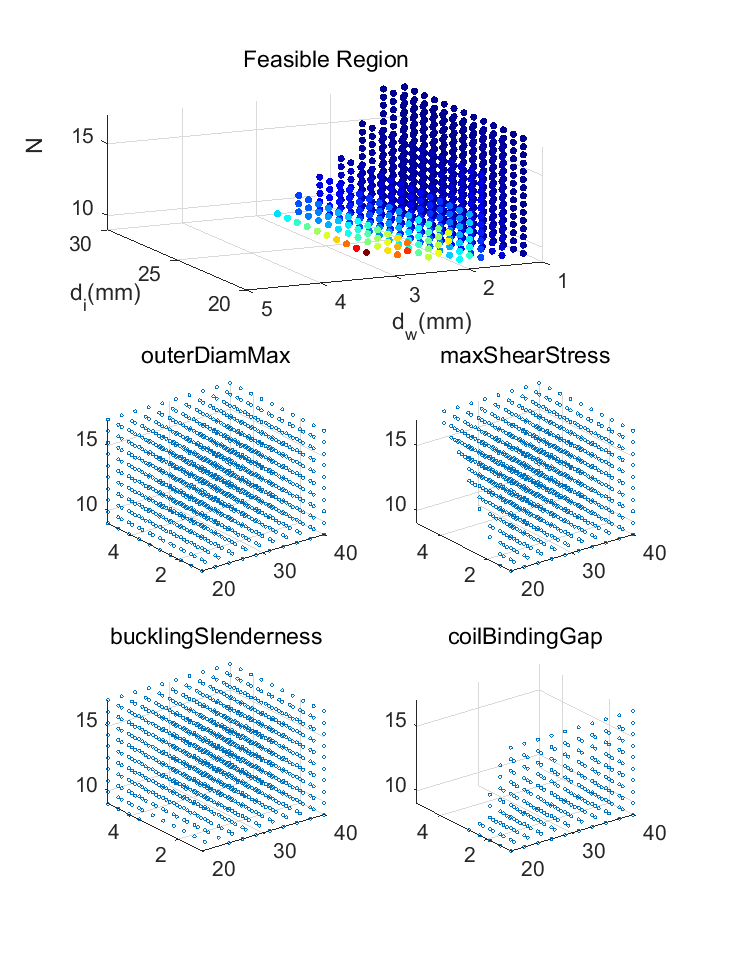
\includegraphics[scale=.5]{Case_56_38910new.eps}\end{center}
		 \caption{Feasibility region for case 1.}
		 \label{Feasibility region for case 1.}
		 \end{figure}

	
	\subsubsection{Sensitivity}
	
\begin{center}
	 \begin{tabular}{| c  | c |  }
	 	\hline Variable & Sobol Index\\
	 	\hline $d_{i}$ & 0.16 \\
		\hline $d_{w}$ & 0.61  \\
		\hline $N_{t}$ & 0.02 \\ 
		\hline
	 \end{tabular}
\end{center}

From the sensitivity indices, it can be observed that all the design variables have significant influence on the objective function; therefore no dimension reduction is implemented for design optimization. 

	\subsubsection{Optimization}
	
	As stated in Section \ref{sec:Optimization}, DIRECT algorithm is used for optimization and the optimum design point is obtained as 
	\begin{center}
	$\mathbf{x_{opt}} =
	\left[
	\begin{array}{c}
	 	 .03 \\
	 	 .001 \\
		 17    \\ 
		
	 \end{array}
	 \right]
$	
\end{center}
    Therefore, the optimum inner diameter($d_{i}$), optimum wire diameter ($d_{w}$), and optimum number of coils ($N_{t}$) are $30 mm$, $1 mm$ and $17$ respectively.
		
\newpage
%-----------------------------------Computational Experiments.2-----------------------------------%
\subsection{Case 2:}
\label{subsec:Case2}
%Case_56_3891011

\begin{description}[leftmargin=!,labelwidth=\widthof{\bfseries State Variables:}, labelindent = 1cm]
	\item[Objectives:] Minimize spring rate and spring index.\\
	\item[Constraints:] Relation on inner, wire, and outer diameter, diametral expansion, coil binding gap, buckling slenderness, and maximum shear stress, stress relaxation. \\
	\item[State Variables:] $d_{i}$, $d_{w}$, and $N_{t}$ \\
\end{description}

	\subsubsection{User Input}
	
\begin{center}
	 \begin{tabular}{| c  | c |  }
	 	\hline Name & Value\\
	 	\hline G & 77 GPa \\
		\hline UTS & .7GPa \\
		\hline $g_{min}$ & .5 mm\\ 
	 	\hline $k_{max}$ & 20\\
		\hline $C_{max}$ & 10\\
		\hline $L_{free}$ & 85.5 mm\\
		\hline $L_{hard}$ & 20 mm\\
		\hline Norton Bailey $c$& $ 3.5 \times 10^{-6}$ \\
		\hline Norton Bailey $n$ & 1.5\\
		\hline Norton Bailey $k$ & 1 \\
		\hline Minimum Stress Relaxation & 0.85\\
		\hline Deflection $s$ & 30 mm\\
		\hline Time Stress Relaxation $t$  & $3 \times 10^{6}$\\
		\hline Stress Relaxation $G_{sr}$ & 60 GPa\\
		\hline
	 \end{tabular}
\end{center}

	\subsubsection{Problem Definition}
	
	\centerline{$Min$ \hspace{2 mm}$0.5 \times(k/k_{max}) + 0.5 \times (C/C_{max})$}
	\begin{center}such that \end{center}
	\centerline{$d_{i} + 2 \times d_{w} \leq 60e-3$}
	\centerline{$g_{min} - \dfrac{L_{hard} - N_{t}d_{w}}{N_{t}-1} \leq 0$}
	\centerline{$\dfrac{L_{free}}{d_{i} + d_{w}} - \pi \sqrt{\frac{2(2 \nu + 1)}{\nu + 2}} \leq 0$}
	\centerline{$d_{\text{w}} + \sqrt{(d_{\text{i}} + d_{\text{w}})^{2} + \frac{p^{2} - d_{\text{w}}}{\pi^{2}}} - d_{o}^{max} < 0$}
			
	\centerline{$\frac{G(L_{free} - L_{hard})}{4 \pi (N_{t} - 2) } \left[\frac{d_{w} (4d_{i}^{2} + 9.46d_{i} 
d_{w} + 3 d_{w}^{2})}{d_{i}(d_{i}+d_{w})^{3}}\right] - UTS \leq 0$}
    \centerline{$20e-3 \leq d_{i} \leq 30e-3$}
    \centerline{$1e-3 \leq d_{w} \leq 5e-3$}
    \centerline{$9 \leq N_{t} \leq 17$}
    
 \centerline{${4\over G_{sr}\theta d_w^4}\int_0^{d_w} r^2 \left( (G_{sr}\theta r)^{-n} + {c\over k} G_{sr}nt^k \right)^{-{1\over n}} \,\mathrm{d} r \ge .85$}
%\begin{center} where $\theta = {2s\over \pi N_a (d_i+d_w)^2}$ \end{center}
\centerline{where $\theta = {2s\over \pi N_a (d_i+d_w)^2}$}

\begin{flushleft}
Similar to the first case study, $\textbf{x}$ is a $3 \times 1$ vector, where $x_{1}$, $x_{2}$ and $x_{3}$ represents the inner diameter ($d_{i}$), wire diameter ($d_{w}$) and total number of coils $N_{t}$ respectively.
\end{flushleft}


\newpage
\subsubsection{Feasibility}
	
			\begin{figure}[H]
		 \begin{center}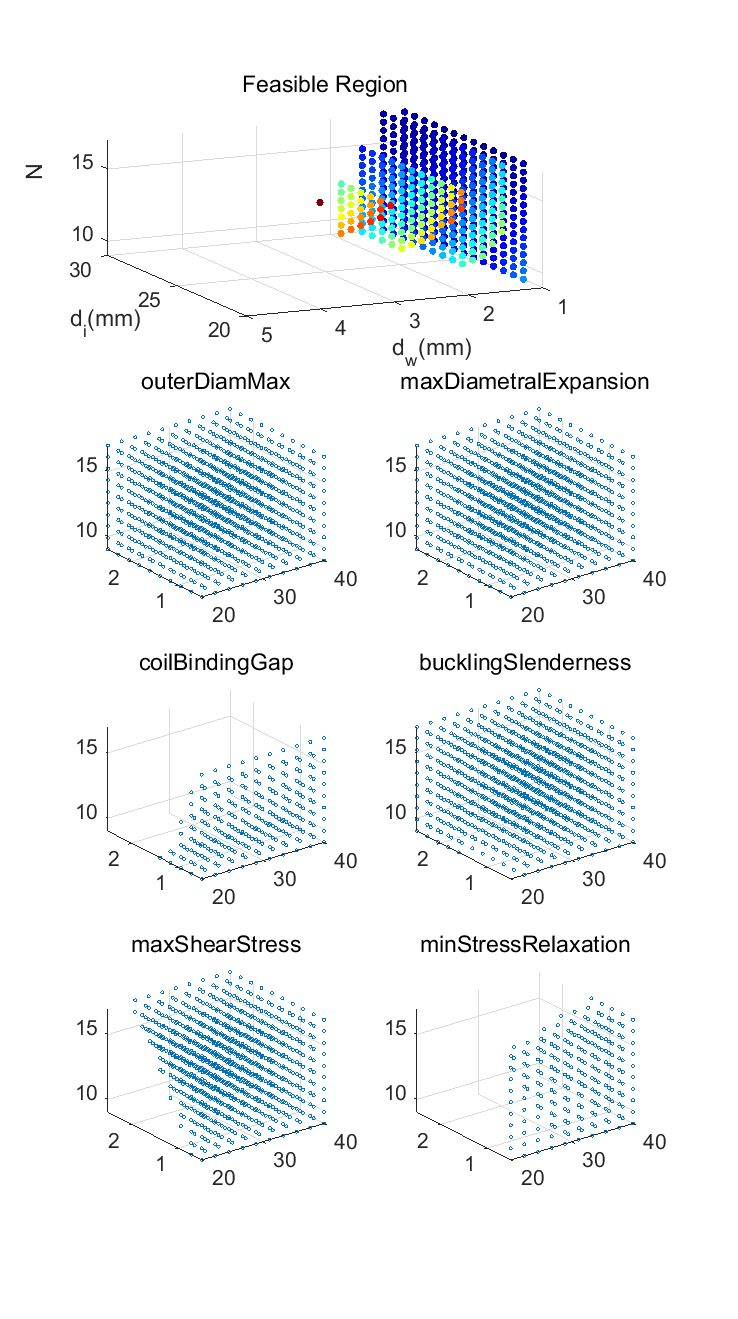
\includegraphics[scale=.5]{Case_56_34891011new.eps}\end{center}
		 \caption{Feasibility region for case 1.}
		 \label{Feasibility region for case 1.}
		 \end{figure}
		 
\subsubsection{Sensitivity}		
 
		 \begin{center}
	 \begin{tabular}{| c  | c |  }
	 	\hline Variable & Sobol Index\\
	 	\hline $d_{i}$ & 0.19 \\
		\hline $d_{w}$ & 0.64  \\
		\hline $N_{t}$ & 0.02 \\ 
		\hline
	 \end{tabular}
\end{center}

From the sensitivity indices, it can be observed that all the design variables have significant influence on the objective function; therefore no dimension reduction is implemented for design optimization. 


\subsubsection{Optimization}
	
	As stated in Section \ref{sec:Optimization}, DIRECT algorithm is used for optimization and the optimum design point is obtained as 
	\begin{center}
	$\mathbf{x_{opt}} =
	\left[
	\begin{array}{c}
	 	 .03 \\
	 	 .001 \\
		 17    \\ 
		
	 \end{array}
	 \right]
$	
\end{center}
    Therefore, the optimum inner diameter($d_{i}$), optimum wire diameter ($d_{w}$), and optimum number of coils ($N_{t}$) are $30 mm$, $1 mm$ and $17$ respectively. Even though an additional constraint about stress relaxation is added, the optimum solution remained the same. Therefore, the assumed stress relaxation constraint does not influence the optimum solution.
    
%-----------------------------------------------------------------Summary and Future Work-----------------------------------------------------------------%
\section{Summary and Future Work}
\label{sec:Summary}

We developed an intelligent tool for the design of helical compression springs. The key highlights of this tool are: One, it allows for flexible optimization, which enables design of springs with interchanging objective functions and constraints. Two, it can incorporate stress relaxation in the design process, which to our knowledge has never been done. Three, it provides a feasibility design space given the constraints. Four, it can provide the global sensitivity indices of the design variables to the objective function. 

Some limitations of the approach outlined are as follows. The choice of optimization and sensitivity analysis are fixed, however, they are modularized to allow a different optimization routine and sensitivity analysis to be incorporated. Given the amount of flexibility that is enabled, a user will have to be able to decide if a infeasible solution is due to user error. 

More analysis of the stress relaxation and creep could result in better performance when using those conditions. Analysis on models of stress relaxation and their performance in our model would be beneficial for both our design, and could further understanding of stress relaxation and creep.

In this work, the DIRECT algorithm for global optimization is used for the design of springs. Also, computational experiments have been carried to perform design optimization considering tolerances in design variables but not incorporated in the design tool; this is an future work of importance. Other future work is to considering faster single-loop techniques, faster analytical and sampling techniques such as First Order Reliability Methods (FORM), and Importance sampling need to be considered

% The key highlights of this tool are (1) Allows for flexible optimization, which enables design of springs with interchanging objective functions and constraints, (2)Can incorporate stress relaxation in the design process, (3) Provides a feasibility design space given the constraints, (4)Provide the global sensitivity indices of the design variables to the objective function. 
% The ability to interchange constraints and objective functions with any number of design variables allows the user the utmost flexibility. With the addition of feasibility and sensitivity analysis it is possible for any configuration of objective function, constraints, and design variables to be analyzed for refinement. The quantification of stress relaxation and creep allow the user a chance to incorporate these properties into any configuration, especially those that have never been tested. The sensitivity indices serves two purposes - help the designer understand which variables have the most influence on the objective function and also help in dimension reduction in the design space for a faster optimization.

%Provide some highlights of object-oriented programming for Spring model design
%
%A couple of sentences of stress relaxation



%In this work, the nested double-loop approach is used for global sensitivity analysis. As the dimension of design variables increases, the nested double-loop approach becomes computationally very intensive. Therefore, more faster single-loop techniques should be considered. Also, reliability analysis within the optimization procedure is carried out using Monte Carlo sampling. As the complexity of the problem increases, in terms of the number of design variables and the number of constraints, Monte Carlo sampling becomes very intensive. Therefore, faster analytical and sampling techniques such as First Order Reliability Methods (FORM), Importance sampling need to be considered.



\section{Appendix}
\label{sec:Appendix}
A rocket mounted spring is expected to deliver normal mechanical output under extreme temperatures. The analysis of creep behavior helps us design a spring to meet the requirements under rough conditions.

Creep is the strain increase under constant stress, usually activated by high temperatures. Three mechanisms have been proposed to account for the phenomenon: dislocation slip and climb, grain boundary sliding and diffusional flow. We focus on the creep caused by the dislocation mechanism. The material's creep tendency is determined by a creep test. During a test, the spring is kept at $0.3-0.5T_m$ ($T_m$ is the melting temperature of the material) and loaded by a constant tensile force.

Conventionally, creep can be divded into $3$ stages. In the first stage (primary/ reduced/trasient) ,the creep strain rate decreases to a certain value(minimum creep rate). The second stage(secondary/steady/stationary creep) is characterized by a nearly constant creep rate(minimum creep rate). In the third stage(tertiary creep), the creep strain rates increases rapidly and leads to rupture. The first stage is usually reversible with time after unloading, while the second/third ones are not. Since the primary creep occurs in a short duration and the tertiary one leads quickly to rupture, the secondary creep is under most serious consideration in many engineering designs.

Another common test to determine the material's susceptibility to high temperature is called stress relaxation. During the test the load is continuously decreased in such a way that the initial strain remains constant. The mechanism is more or less the same as that of creep.

\subsection{Creep rate law of material}
\label{sec:Creep}
The starting point is the assumption that the creep rate may be described as a product of three separate functions of stress, temperature and time
\[
\epsilon_{cr}(\sigma,T,t)=f_\sigma (\sigma) f_T(T) f_t(t)
\]
The widely used functions of stress $f_\sigma(\sigma)$ are (\cite{Creep}):

\begin{tabular}{ll}
$a\sigma^n$ & Norton, 1929, Bailey, 1929 \\
$b\left( \exp{\sigma\over \sigma_0} -1 \right)$ & Soderberg, 1936 \\
$a\mathop{sinh}{\sigma\over \sigma_0}$ & Prandtl, 1928, Nadai, 1938, McVetty, 1943\\
$a_1\sigma^{n_1} + a_2 \sigma^{n_2}$ & Johnson et al., 1963 \\
$a\mathop{sinh} \left( {\sigma\over \sigma_0}\right)^n$ & Garofalo, 1965
\end{tabular}

where $a,b,a_1,a_2,\sigma_0,n_1,n_2$ are material constant. The dependence on the temperature $f_T(T)$ is usually expressed by the Arrhenius law
\[
f_T(T) = \exp \left( {-Q\over RT}\right)
\]
where $Q$ and $R$ denote the activation energy and the Boltzmann's constant.

The time dependence part $f_t(t)$ is assumed to be (\cite{Ch2000}):

\begin{tabular}{ll}
$t$ & secondary creep \\
$bt^m$ & Bailey \\
$(1+bt^{1/3})\exp{kt}$ & Andrade\\
$\sum_j a_j t^{m_j}$ & Graham and Walles
\end{tabular}

For simplicity, we are going to only use the Norton-Bailey law and ignore any dependence on the temperature since the temperature is constant.
\section{Stress relaxation of helical spring}
The following section is based on the paper(\cite{Relaxation1}). Due to conservation of the total shear strain, the sum of the creep strain $\epsilon_{cr}$'s rate of change and that of elastic shear strain $\epsilon_{el}$ is zero:
\[
\dot{\epsilon}_{cr} + \dot{\epsilon}_{el} = 0
\]
Dot is meant as differentiation in time. The elastic shear strain is related to the shear stress by shear modulus $G$: $\epsilon_{el} = \sigma/G$ and taking the derivative with time on both sides, we arrive at
\[
\dot{\epsilon}_{el} = \dot{\sigma}/G
\]
According to Norton-Bailey law(also known as time hardening law),
\begin{equation} \label{eq:N-B}
\dot{\epsilon}_{cr}(t)=c\sigma^{n+1} t^{k-1}
\end{equation}
where $c$ is the shear strain rate, $n,k$ are temperature dependent material constants.

Substituting the above two equations to the conservation law,
\begin{equation} \label{eq:diff}
\dot{\sigma}(t)/G+c\sigma(t)^{n+1} t^{k-1}=0
\end{equation}
The initial condition is
\[
\sigma (0) = G\theta r
\]
where $\theta$ is the initial twist angle per unit length, $r$ the radius of wire.

\[
\sigma = \left( (G\theta r)^{-n} + {c\over k} Gnt^k \right)^{-{1\over n}}
\]

The torque can be written as
\begin{align*}
&M(t) = 2\pi \int_0^{d_w} r^2 \sigma(r,t)\,\mathrm{d} r\\
&M(0)={1\over 2} G\pi\theta d_w^4
\end{align*}
where $d_w$ is the wire diameter.

Since the spring load is linearly related the torque $P_z(t)\propto M(t)$, given the constant deflection $s$,
\[
{P_z(t)\over P_z(0)} = {M(t)\over M(0)} = {4\over G\theta d_w^4}\int_0^{d_w} r^2 \left( (G\theta r)^{-n} + {c\over k} Gnt^k \right)^{-{1\over n}} \,\mathrm{d} r
\]
where
\[
\theta = {2s\over \pi N_a ((d_i+d_o)/2)^2}
\]
The integral has no endpoint singularity and can be integrated to high order precision using the Gauss quadrature formula. The closer this quantity is to $1$, the better the spring quality is. We notice that a seemingly simpler form has been presented in the paper.
\[
{}_{2}F_1 \left( {4\over n},{1\over n};{4+n\over n};{c\theta^n G^{n+1} n t^k\over k} {d_w^n\over 2^n}\right)
\]
which we find to yield unrealistic values due to divergence issues.

\subsection{Stress relaxation of helical spring}
\label{sec:Relaxation}

Due to conservation of the total shear strain, the sum of the creep strain $\epsilon^{cr}$'s rate of change and that of elastic shear strain $\epsilon_{el}$ is zero:
\[
\dot{\epsilon}_{cr} + \dot{\epsilon}_{el} = 0
\]
The elastic shear strain is related to the shear stress by shear modulus $G$:
\[
\epsilon_{el} = \sigma/G
\]
and therefore
\[
\dot{\epsilon}_{el} = \dot{\sigma}/G
\]
According to Norton-Bailey law(also known as time hardening law),
\begin{equation} \label{eq:N-B}
\dot{\epsilon}_{cr}(t)=c\sigma^{n+1} t^{k-1}
\end{equation}
where $c$ is the shear strain rate, $n,k$ are temperature dependent material constants.

Substituting the above two equations to the conservation law,
\begin{equation} \label{eq:diff}
\dot{\sigma}(t)/G+c\sigma(t)^{n+1} t^{k-1}=0
\end{equation}
The initial condition is
\[
\sigma (0) = G\theta r
\]
where $\theta$ is the initial twist angle per unit length, $r$ the radius of wire.

\[
\sigma = \left( (G\theta r)^{-n} + {c\over k} Gnt^k \right)^{-{1\over n}}
\]

The torque can be written as
\[
M(t) = 2\pi \int_0^{d_w} r^2 \sigma(r,t)\,\mathrm{d} r ={}_{2}F_1 \left( {4\over n},{1\over n};{4+n\over n};{c\theta^n G^{n+1} n t^k\over k} {d_w^n\over 2^n}\right) M(0)
\]
where $d_w$ is the wire diameter.

Since the spring load is linearly related the torque $P_z(t)\propto M(t)$, given the constant deflection $s$,
\[
{P_z(t)\over P_z(0)} = {}_{2}F_1 \left( {4\over n},{1\over n};{4+n\over n};{c\theta^n G^{n+1} n t^k\over k} {d_w^n\over 2^n}\right)
\]
where
\[
\theta = {2s\over \pi N_a ((d_i+d_o)/2)^2}
\]
The closer this quantity is to $1$, the better the spring quality is.

\subsection{Creep of helical spring}
This section is based on the paper(\cite{Relaxation3}). The starting point is still the Norton-Bailey law (\ref{eq:N-B}). There is naturally another way to write the shear strain rate:
\[
\dot{\epsilon}_{cr} = \dot{\theta} r = {8\dot{s} r\over \pi N_a (d_i+d_o)^2}
\]
We obtain $\sigma$ from substiting the above equation into Norton-Bailey law. Given the constant spring force $P_z^0$,
\[
P_z^0{d_i+d_o\over 4}=M(0)=2\pi\int_0^{d_w} r^2 \sigma(r,t)\,\mathrm{d} r
={\pi\over 4}{n+1\over 4+3n}\left( {8d_w^{4+3n}\dot{s} \over t^{k-1} (d_i+d_o)^2 \pi N_a c (d_i+d_o)^2} \right)^{{1\over n+1}}
\]
It can be deduced that the spring length $s$ follows
\[
s(t) = s(0) + \left( {(d_i+d_o)P_z^0\over \pi}{4+3n\over n+1} \right)^{n+1} {\pi (d_i+d_o)^2 N_a c\over 8kd_w^{4+3n}} t^k
\]
where $s(0)$ is the initial spring length. The less the difference of the spring length $s(t)-s(0)$, the better the spring quality is.
 
 \cite{Ch2000} \cite{Relaxation1} \cite{Relaxation2} \cite{Relaxation3} \cite{Creep} 
\subsection{Analysis of stress relaxation and creep models}
\label{sec:stressanalysis}




\vfill\pagebreak


	
	\bibliographystyle{ieetr}

\bibliography{MyBib}



\end{document}

